\documentclass{sbir}

\usepackage{fixme}
\fxsetup{
    status=draft,
    author=,
    layout=margin,
    theme=color,
    targetlayout=color
}

%%%%%%%%%% Proposal-specific Information %%%%%%%%%%%%%%%
\company{AHS Engineering Services}
\proposaltitle{WARDEN: Demonstrating and Defining Secure Efficient Cross-domain Protocols}
\topicnum{AF13-AT08}
\proposalnum{F13A-T08-0015}
\proposaltype{STTR Phase I Proposal}
%%%%%%%%%%%%%%%%%%%%%%%%%%%%%%%%%%%%%%%%

\begin{document}

%%%%% List the FiXme annotations  %%%%%
%\listoffixmes
%\newpage
 
%%%%%  Roman numerals for TOC  %%%%%
%\pagenumbering{roman}
%\tableofcontents
%\newpage
 
%%%%% Set the page number that the main proposal will start on %%%%%%
\pagenumbering{arabic}
\pagestyle{proprietary}

\cfoot{
{\color{LeTigre}\vspace*{-1.1in}{\it\small{This proposal includes data that shall not be disclosed outside the Government and shall not be duplicated, used, or disclosed-in whole or in part-for any purpose other than to evaluate this proposal. If, however, a contract is awarded to this offeror as a result of-or in connection with-the submission of this data, the Government shall have the right to duplicate, use, or disclose the data to the extent provided in the resulting contract. This restriction does not limit the Government's right to use information contained in this data if it is obtained from another source without restriction. The data subject to this restriction are contained in pages 1--5 and 7--20.}~\\
\scshape\fromproposaltitle}~\\ \rm\thepage }
}

\sbirsection{Identification and Significance of the Problem or Opportunity}
{The AHS Team proposes to develop and deliver a functional prototype system, hereafter termed WARDEN,  coupled with a reference architecture demonstrating cross-domain information protocols with known security characteristics. This system, based on our extensive and published previous work with usage management and policy-centric information networks,  will be rigorously characterized from an engineering and theoretical perspective to clarify the security of defined protocols and susceptibility to covert channel communication. The protocols themselves will be clearly defined and will be implemented within the system as a reference for other engineers as needed. These protocols and their implementation provide clear benefits to potential adopters, including but not limited to both the healthcare information management industry and the defense industrial base.}

%%%%%  Evaluation Criteria box, use \begin{evalbox} \end{evalbox}, \evalhdr, \begin{evalitemize}, and \end{evalitemize}  %%%%% 	
\begin{evalbox}
\evalhdr{Innovative:}
  \begin{evalitemize}
     \item Addresses the WARDEN problem via a proven policy-based usage management framework.
     \item Underlying logic framework supports sophisticated formal reasoning capabilities.
  \end{evalitemize}
\evalhdr{Sound Technical Approach:}
  \begin{evalitemize}
     \item Based on open standards and open source product development.
     \item Leverages AHS's demonstrated work in policy-based usage management.
  \end{evalitemize}
\evalhdr{Qualifications:}
  \begin{evalitemize}
     \item AHS Co-PI has significant experience with SBIR/STTR development and technology transition.
     \item UNM Co-PI has considerable expertise in information security and usage management.
     \item SNL Co-PI has extensive knowledge in information-centric networks, and software engineering and architecture.
  \end{evalitemize}
\evalhdr{Benefits:}
  \begin{evalitemize}
     \item Dynamically and securely share information with properly credentialed users based upon policy.
     \item An agile usage management framework that scales to the enterprise.
  \end{evalitemize}
\evalhdr{Commercialization:}
  \begin{evalitemize}
     \item Deployable in multiple industries with sensitive information.
  \end{evalitemize}
\end{evalbox}

\paragraph{Executive Summary}
\paragraph{The Problem.} In the past, information flow has been retarded by time-consuming release procedures and rampant over-classification, leading to a lack of information when warfighters need it most. Current structures in place to protect sensitive information rely on time-consuming human review, and place heavy responsibilities upon those given access to such sensitive material. The penalties for inadvertent sensitive information disclosure, though appropriate, have the side effect of encouraging reviewers to place material at the highest justified classification level. This has also led to difficulty partitioning system deployments, as redundant systems need to be installed and supported in multiple different security domains, leading to increased costs.

The goal of this research and development effort is to characterize cross-domain information flow protocols for security, including analysis for possible covert channel communications, building reference implementations of promising candidates. The reference information transfer network (i.e., WARDEN) will demonstrate possible practical application of these protocols and associated techniques. 

Future systems should be able to partition work and information into discrete bundles with known security characteristics that can be processed and stored in environments suitable for those packages. Furthermore, these disparate systems should be able to securely collaborate across security domains, working toward common goals. Communication and collaboration must be facilitated by coordinating information and processing routers distributed throughout the network fabric, protecting and maintaining the consistency of sensitive information as appropriate.

This kind of system enables information dissemination throughout the warfighter's enterprise, supporting timely delivery of information to those who need it, fulfilling an organization's responsibility to share information with those who need it. This kind of collaboration lowers costs, increases system utility, and ultimately gets information to those who need it so they can use it.
\clearpage
\cfoot{\color{LeTigre}\vspace*{-1.25em}{\scshape\fromproposaltitle}~\\ \rm\thepage~\\ 
\it{Use or disclosure of data contained on this page is subject to the restriction on the first page of this volume.}}

\paragraph{The Solution Objective.} The AHS Team, composed of personnel from AHS Engineering Services, the University of New Mexico (UNM), and Sandia National Laboratories (SNL), proposes to design, prototype, and develop WARDEN, a provably secure information management network. WARDEN will extend our SMASHUP framework, a highly flexible usage-managed information-centric overlay network built to protect information transmitted through dynamically configured information domains. SMASHUP has been used in standalone configurations and integrated with both cloud computing infrastructures and the Distributed Common Ground System's (DCGS) Integration Backbone (DIB). Protocols implemented within WARDEN will have specific provable security characteristics coupled with a clear understanding of covert channel potential limiting or eliminating any possible inadvertent information leakage.
\begin{center}
\vspace{-12pt}
   \fcolorbox{BlueSteel}{Magnum}{
         \begin{minipage}[t]{0.9\textwidth}
Sandia National Laboratories is pleased to partner with AHS Engineering Services and the University of New Mexico to further the state of the art in cross-domain technology via the work outlined in this STTR. SNL currently plans to provide material support, including but not limited to computational time and equipment as needed for Phase I work. SNL will be further involved in Phase II, providing not only computational resources but also personnel at a level commensurate with the level of work outlined in the future Phase II proposal. Specifically, Dr. Chris Lamb will work in his capacity as a Research Professor in Phase I, and then begin to spend additional time on this effort as a Principal Scientist at SNL starting in Phase II.
         \end{minipage}
      }
\end{center}

\paragraph{Our Approach.} 
Future workflows will span different security domains. All the domains will contribute data and processing cycles to common solutions, unified via some kind of service-oriented conceptual design. In this kind of system, data and the results of data processing will be transferred between dedicated information guards that will enforce classification standards over transferred information.

\begin{figure}
\vspace{-0.2in}
\centerline{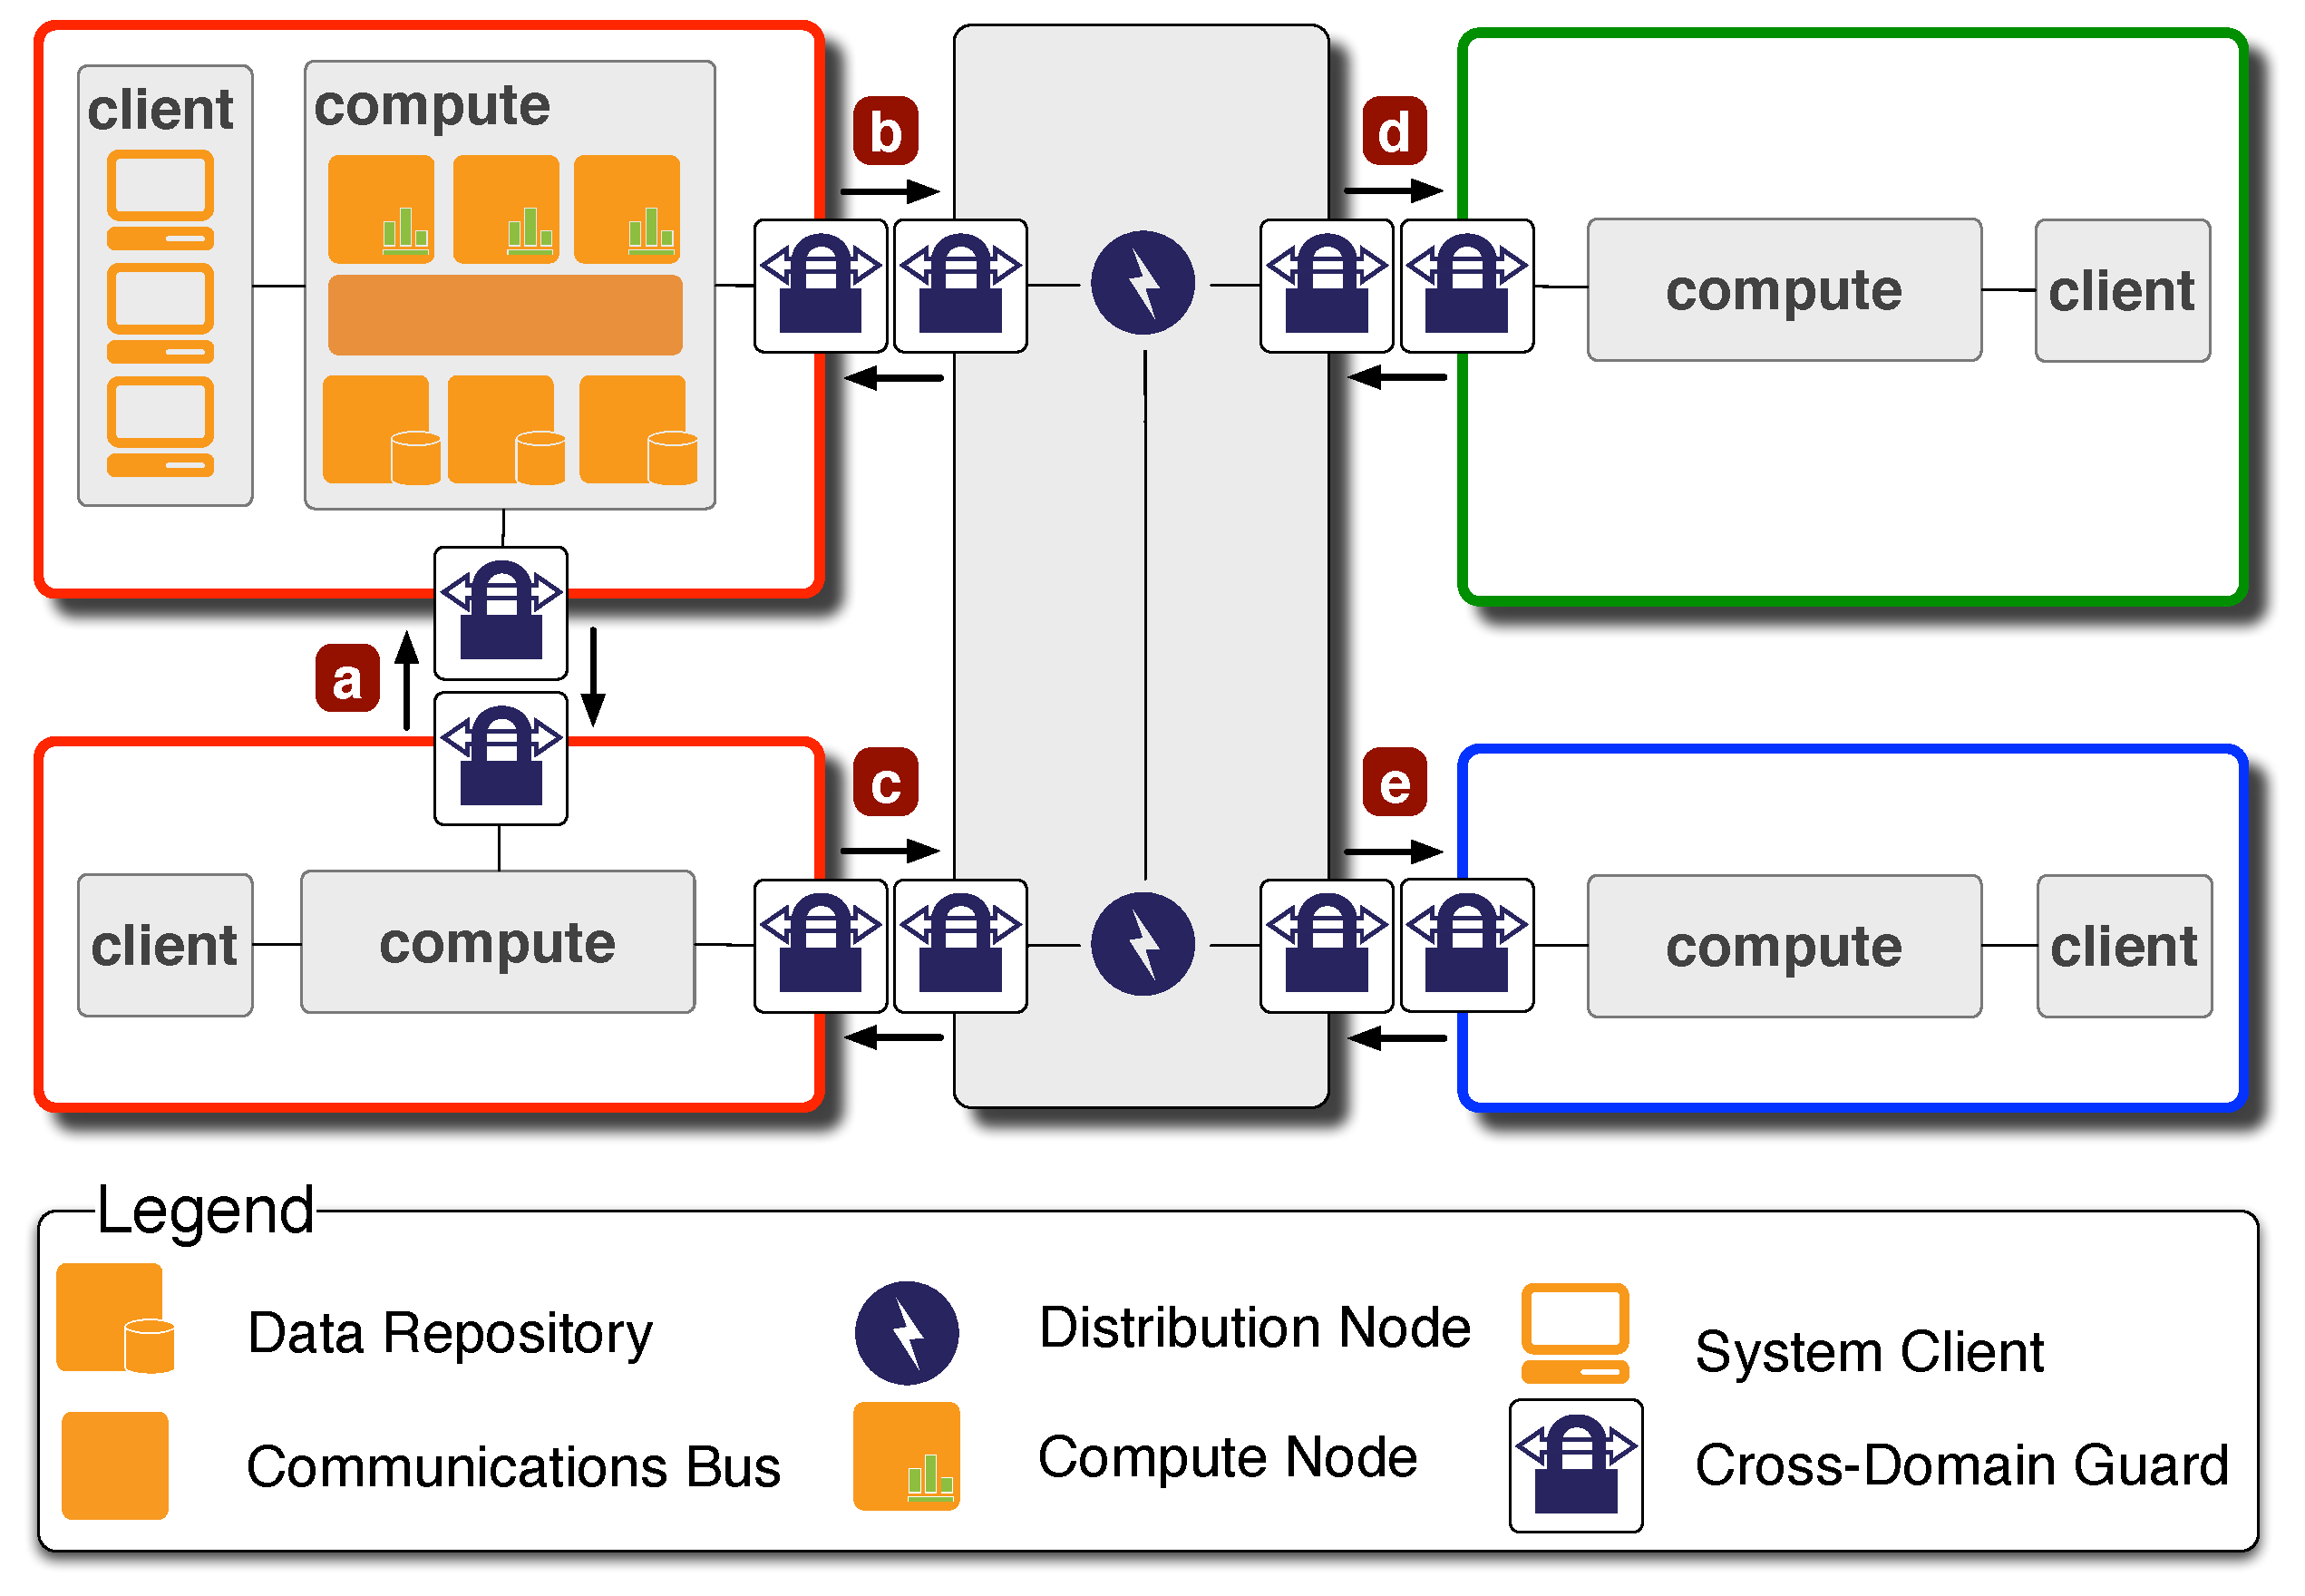
\includegraphics[width=6in]{./images/warden-conops.pdf}}
\vspace{-0.1in}
\caption{The concept of operations for the WARDEN system.}
\label{conops}
\end{figure}

Figure ~\ref{conops} embodies this kind of environment. Here, we have different security domains (highlighted in red, blue, and green) which can all work together to provide computational services to integrated clients via either a common information backbone or direct domain communication. In this envisioned environment, information passing through the guards (a, b, c, d, and e) is strictly managed and controlled to avoid information leakage. To avoid malicious exfiltration, these guards must also have clearly understood and minimized covert communication capabilities.

Our proposed work will enable these kinds of cross-domain workflows by rigorously defining covert channel capabilities for various guard communication protocols, classifying possible protocols into a taxonomy, and providing reference implementations of the most promising protocol candidates in a framework representative of the notional architecture shown in Figure ~\ref{conops}.

\paragraph{Vision and End-State.} The end state of our Phase I research project will be the production of the WARDEN architecture and initial prototype that demonstrate the feasibility of our approach for success during Phases II and III. Specifically the prototype will demonstrate protocols with known security characteristics in operation between and through cross-domain guard nodes facilitating collaborative, cross-domain workflows. The technology readiness level (TRL) will be established at the conclusion of Phase I.

\paragraph{Background and Need}~\\
Federal agencies are transitioning from a need-to-know model of information dissemination, where users need to provide a demonstrative need to have access to information in order to be granted access, to a more open responsibility-to-provide model. While need-to-know is being modified, it is not being removed as a requirement. Rather, agencies need to heed the notion responsibility-to-provide  while still supporting robust need-to-know controls -- neither can be acceptably violated in today's environment. These principles affect everyone with a security clearance and all organizations that manage classified data.

\sbircallout{The technical challenges.}{Current systems provide static, one-size-fits-all functionality for operational information delivery. This is unsuitable for today's dynamic operational environments that change rapidly and unexpectedly. Next-generation messaging solutions for the warfighter must incorporate dynamic security, responsive cross-domain information dissemination, and the ability to adapt to chaotic technical operating environments.}

These principles become difficult to rectify in today's computational environments. The primary issue is moving classified information to an an environment at a lower classification level. This downgrading currently involves human review of data objects, in which reviewers redact sensitive information. Not all content in classified documents is necessarily sensitive, so when going through this kind of downgrading process, reviewers remove the sensitive content from the documents, leaving non-sensitive content appropriate for distribution. This process is generally referred to as sanitizing a document. This primarily impacts document downgrades, but can also impact moving information from one compartment to another, where compartments are separate categories of information within a single classification level.

This review system is an artifact of how sensitive information has traditionally been managed. To this day, computer systems are classified by the kind of information they can contain based on one of a variety of possible models. These models fall into two basic categories, government-sponsored standards or international, open standards. Current governmental standards include the Trusted Computer System Evaluation Criteria, the Information Technology Security Evaluation Criteria, and the Canadian Trusted Computer Product Evaluation Criteria. These have all been sponsored and developed by the defense departments of the United States, Great Britian, and Canada, respectfully. The most current international standard addressing system security is the Common Criteria, sponsored by the International Organization for Standardization (ISO). Labeled ISO/IEC 15408, the Common Criteria generalize and extend the principles established in previous, government-sponsored standards.

All of these standards group systems into categories based on security profiles that enable acceptable sensitive processing. Systems must be accredited to handle sensitive information, and the more sensitive the information, the more secure the processing system must be. This has led to a coupling of systems and content, rather that users and content. Today, a given system is accredited to handle information of a certain sensitivity first, and then users can be granted accounts on that system giving them access to sensitive information based on an external vetting process. In this scenario, users are given access to systems, not content. Content access is a side-effect of system access.

A better approach is to evaluate suitability based on the content requested rather than the system a user is accessing. In order to do this, we must have some way to describe what that sensitive data is. This implies the existence of specific ontologies that describe the information we process, as well as some mechanism to rectify them when managing content with different origins. This also implies a shift in applied security models, shifting from Bell-LaPadula and Biba models to more modern models like Brewer-Nash and Clark Wilson. In any and all of these cases, possible covert communications from the involved systems must be minimized.

\paragraph{Challenge 1: Protocol class feature identification.}
In our previous work with SMASHUP, we identified three basic classes of semantic protocols supporting cross-domain information exchange. These basic protocols supported workflow-centric information flow through guard routers, and had specific advantages and disadvantages and different levels of expressive complexity and power.

The first approach is hierarchy-based, and is closest to current production systems. In this scheme, we group content based on a single tag that corresponds to a hierarchy of sensitivity. The sensitivity hierarchy is an ordered, traditional security lattice, allowing us to easily make decisions about access. Though this approach is computationally simple, it does not however provide any insight into why content is classified at a particular level, nor does it support any kind of content-based access adjudication.

The second approach uses a hierarchy with attached semantic metadata attributes. Here, we maintain a totally ordered set of classifiers, but we also maintain semantic information describing specifically what it means to be grouped within one of the classifiers. This way, we can rectify content described under two different classification hierarchies. For example, if one artifact is classified under hierarchy A, and another under hierarchy B, with this additional semantic information we are able to determine specifically what it means to be classified under these hierarchies, and manage an aggregate content object formed from both artifacts more effectively.

The final approach is purely attribute based, where content and user permissions are both described with semantic information. In this case, we no longer maintain a hierarchy of classifiers. Rather, we simply maintain semantic metadata associated with both users and artifacts, and rectify access to artifacts accordingly.

These protocols are samples of the kinds of protocol classes needed in production information exchange environments. Not only does information need to be rectified between domains for evaluation when transferred through a guard, guarding systems must handle query processing as well --- bi-directional traffic through a guard protecting domains with specific and conflicting need-to-know requirements is common and adds additional complexity to the information analysis process. Developed protocols must also  address degrees of information known about collaborating domains as not all information about transferred information is guaranteed to be available, particularly in operational environments deployed in-theater.

\paragraph{Challenge 2: Protocol development and analysis.}
A cross-domain protocol must generally define the sequence of messages between the guard and involved end-point domains and what information is transmitted in each message. The sequence of messages must allow the system to transmit data in an efficient manner while suppressing any possible covert channel. 
The communications must also give the guard the information it needs to make a cross-domain decision. The required information includes the ontologies of the two domains, the policy set of the requested information, and any meta-policy sets of the requested information.

%A possible sequence could be:
%\begin{enumerate}
%\item Request for information is sent to guard.
%\item The guard retrieves the ontology of the domain that the requested information is in.
%\item The guard retrieves the policy set of the requested information.
%\item The guard retrieves the ontology of the domain that made the request.
%\item Ontological rectification is performed.
%\item Meta-policy enforcement. \hl{<<Incomplete sentence.>>}
%\item The policy set is modified if necessary.
%\item Content is removed or protected if necessary.
%\item The guard sends a message back to the domain that made the request.
%\item The content is moved if allowed.
%\end{enumerate}

Policies can be aggregated into combined policy that protects content at a level coherent with all expressed information protection requirements. Each protocol has specific timing and storage characteristics that could be exploited to develop a covert channel. As such, each protocol in each class must be analyzed for possible covert channel exploitation, and the results generalized for each class to extract possible class-centric characteristics. This covert channel analysis must be rigorous and contribute to the development of a taxonomy of possible classes of cross-domain protocols for information exchange. This taxonomy is vital to allow the identification of possibly overlooked classes and class members, as well as to categorize the most advantageous classes for protocol implementation and eventual deployment.

%\paragraph{Challenge 3: Protocol selection and development.}
%Once protocols have been developed and salient features identified and analyzed, the protocols must be developed and exercised in environments reflecting the operational reality of today's forces to verify ability to implement. These reference implementations serve to provide a springboard for our team as we move into Phase II work with these systems. 
%
%Furthermore, implementing these protocols in current realistic systems helps identify potential protocol problems as soon as possible as well. As protocol errors are discovered farther down the development lifecyle, they become more expensive to fix. Finding these problems as soon and as possible drastically lowers costs associated with defect repair. \hl{<<This does not sound like a challenge, but a task.>>}

\paragraph{Meeting the challenges.} By meeting the above challenges, we will create a clearly organized taxonomy of potential cross-domain protocols. This taxonomy will be characterized from a covert communications perspective, giving the project sponsor point of contact (POC) unique insight into different types of protocols and their advantages and disadvantages. Furthermore, reference implementations of the protocols will prove that the concepts are in fact implementable and realistic for production systems on today's technology.

\sbirsection{Phase I Technical Objectives}
{The project challenges motivate our technical objectives. By meeting these objectives, we will develop a taxonomy of protocols evaluated for covert communications potential with reference implementations, positioning this project for future Phase II work.}

\paragraph{Objective 1: Define reference architecture.} First, we will define a reference architecture that will use our protocols for cross-domain information exchange. This reference architecture will be a living description of the target environment of developed protocols, and will evolve over the course of Phase I as we identify shortcomings via defining potential protocols and protocol classes. This will help frame our thinking around cross-domain information exchange and help us clearly communicate about candidate protocols and protocol classes. Furthermore, this will help our customers and other interested organizations implement similar systems if necessary, and will help us and other potential involved parties later in Phase I prototyping and Phase II development.

\paragraph{Objective 2: Define protocol classes.} Once we have defined a suitable reference architecture, we will begin to define specific protocols that we could use for information exchange within that reference architecture that adhere to defined information protection requirements. We will group these protocols into specific protocol classes, and organize those classes into a clear taxonomy. These classes are vital to identification of specific features associated with common approaches, and the taxonomy will be indispensible in later analysis of the discovered protocol classes for completeness and coverage, where completeness describes the thoroughness of protocols within a class and coverage describes the coverage of the taxonomy with respect to possible known protocol classes. This detailed analysis will enable us to identify both classes and instances of protocols with the highest possible return on development investment, as well as those classes and instances we may have overlooked.

\paragraph{Objective 3: Develop and apply evaluation protocols.} Once we have developed a reference architecture and a taxonomy of protocols and protocol classes, we will begin analysing those protocols for covert channels. This analysis will use the shared resource method, as well as syntactic and semantic information-flow analysis and non-interference analysis. Here, we will specifically identify potential covert-channel communications threat by identifying and rigorously characterizing covert-channel capabilities. This information will then be applied to the taxonomy and all contained elements, clearly characterizing families of protocols with the highest potential security.

\paragraph{Objective 4: Prototype reference architecture and promising protocols.}  Once the taxonomy has been developed and contained elements characterized from the perspective of covert channel potential, we will implement reference examples of promising protocols using our current SMASHUP framework either in a cloud environment or in the DIB, or both. Our current work in multi-domain dynamic information networks gives us a unique platform on which to develop these protocols, allowing us to readily prototype systems in realistic customer environments, ranging from commercial and private cloud computing infrastructures to mission-specific operational information environments.

%\begin{figure}
%  \centerline{\includegraphics[width=4in]{./images/GeoAIDarch.png}}
%  \caption{GeoAID architectural overview.}
%\label{GeoAIDarch}
% \end{figure}

\newpage 
\lfoot{}
\chead{\color{LeTigre}~\\ Topic No: \fromtopicnum}
\cfoot{\color{LeTigre}\vspace*{-1.25em}{\scshape\fromproposaltitle}~\\ \rm\thepage}

\paragraph{Phase I Work Plan Outline (Non-proprietary)}
\paragraph{Scope}~\\
The scope of this effort is to define, organize, and evaluate potential communication protocols supporting workflows that cross security domains. Specifically, these protocols must be characterized from the perspective of possible covert channel communications. Phase I work specifically addresses delivery of cataloged and analyzed protocols including associated proof-of-concept software suitable for verification and validation.

\paragraph{Task Outline} 
\begin{enumerate}
\vspace{-0.1in}
\item {\bf Kickoff Meeting}---We will conduct a meeting with the Sponsor POC within 30 days of contract start.
\item {\bf Requirements Extraction}---We will identify and enumerate system requirements.
\item {\bf Establish Approaches and Architectures}---We will develop a catalog of architectural options including descriptions of the approaches and their advantages and disadvantages.
\item {\bf Define Protocol Classes}---We will identify specific protocols and organize them into potential classes in a taxonomy.
\item {\bf Develop Evaluation Approach and Evaluate Protocols}---We will organize potential covert channel evaluation methodologies and apply them to defined protocols as appropriate.
\item {\bf Prototype System Development}---We will construct a simple framework which is relevant and applicable to the defined protocols. We will verify that research components can be loaded into the framework and run correctly as expected to support evaluation.
\item {\bf Technical Review Meeting}---We will conduct a technical review within six (6) months of project start at a date and time to be coordinated with the Sponsor POC.
\item {\bf System Evaluation}---We will test the developed system and measure key performance attributes.
\item {\bf Reports and Publications}---We will write and submit monthly progress reports and a final report (with SF 298).
\end{enumerate}

\paragraph{Milestone Schedule}~\\
The proposed Phase I effort is scheduled as shown in the Gantt chart in Figure~\ref{Gantt}. The majority of the primary research will be accomplished during the first six months of the Phase I STTR project. The last three months will provide project continuity to Phase II. Work will be performed at AHS Engineering Services facilities and the University of New Mexico in Albuquerque, New Mexico.

\begin{figure}[h]
 \centerline{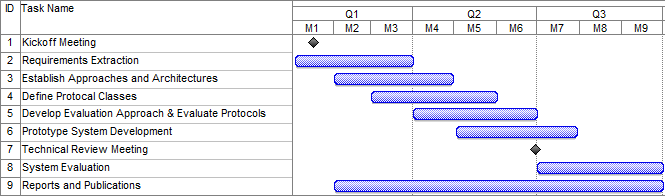
\includegraphics[width=5in]{./images/AF13-AT08_Gantt_Chart.png}}
 \caption{Task and milestone schedule.}
 \label{Gantt}
\end{figure}

\paragraph{Deliverables}
\begin{enumerate}[label=\alph*.] 
\vspace{-0.1in}
\item Kickoff meeting within 30 days of contract start.
\item Progress reports.
\item Technical review within 6 months.
\item Final report with SF 298.
\end{enumerate}

Our work plan is fully responsive to the requirements stated in the published topic. By producing a working proof-of-concept prototype, we will in fact achieve more than the requirements of the topic.

\newpage
\lfoot{\color{LeTigre}\scshape{Proprietary}}
\chead{\color{LeTigre}\scshape{Proprietary}~\\ Topic No: \fromtopicnum}
\cfoot{\color{LeTigre}\vspace*{-1.25em}{\scshape\fromproposaltitle}~\\ \rm\thepage~\\ 
\it{Use or disclosure of data contained on this page is subject to the restriction on the first page of this volume.}}

\sbirsection{Phase I Work Plan}
{This Phase I STTR will result in the definition of the WARDEN technical approach and a software prototype that demonstrates the key aspects of our approach. These results will be in sufficient detail to show proof-of-concept and demonstrate feasibility for the Phase II project and Phase III commercialization.}

\subsection{Key Aspects and Innovation}
AHS Engineering Services is an experienced and highly capable research and development contractor with a proven record of thorough research and innovation, directed toward solving real problems. AHS Engineering Services has been active for over a decade in researching the key technologies required in this effort, and its members have faculty affiliations with the University of New Mexico and the Informatics Research Group, which is highly experienced in the areas of information security and usage management. Our approach integrates proven existing technologies with new innovative approaches. The use and leverage of proven technology provides a sound foundation for our technical approach, reducing technical risk, and providing a platform for our key innovations.

\subsection{Task Summary and Schedule}
The proposed Phase I effort is organized into the tasks shown in the Figure~\ref{Gantt}. Work will be performed at AHS Engineering Services and UNM facilities in Albuquerque, New Mexico.
\vspace{-0.1in}
\begin{center}
\fcolorbox{BlueSteel}{Magnum}{
\begin{minipage}[t]{0.9\textwidth}
\begin{itemize}[labelindent=2em,leftmargin=1.5em,label=$\checkmark$] 
\item Building on information usage management and cloud expertise.
\item Reusing secure cross-domain information-centric systems for data delivery.
\item Mobile-first approach guarantees application-level configurability.
\item Innovative peering approaches to dynamic information delivery needs.
\end{itemize}
\end{minipage}}
\end{center}

\subsection{Task Details and Technical Approach}
The AHS Team will follow an agile software development process for accomplishing the Phase I tasks detailed below. Agile software development is a group of software development methods based on iterative and incremental development, where requirements and solutions evolve through collaboration between self-organizing, cross-functional teams. It promotes adaptive planning, evolutionary development and delivery, a time-boxed iterative approach, and encourages rapid and flexible response to change. It is a conceptual framework that promotes foreseen interactions throughout the development cycle, with a focus on delivering working software~\cite{La:03}.

\heading{Task 1: Kickoff Meeting}
We will hold a kickoff meeting either at the government's site or at UNM, based on Government Sponsor POC preference. In this meeting we will review the proposed technical approach and statement of work and clarify the research sponsor's technical direction.

\heading{Task 2: Requirements Extraction}
In this task, we will identify and enumerate system requirements, aiming for 90\% requirements coverage overall and 100\% requirements coverage with respect to core Phase I protocol functionality. We will name and describe these requirements in a form suitable for future system development and documentation. The primary deliverable from this task will be a document describing these requirements such that the requirements can be traced both forward into protocols, taxonomies, channel analysis, and prototypes, and backward to the initial requirements source. 

\heading{Task 3: Establish Approaches and Architectures}
In this task, we will outline architectural approaches that frame the problem, describe how and why they are applicable, and address how they could be evaluated for potential production use. We will leverage our established usage management technologies and experience to control information flow~\cite{JaLaHe:11,JaLaHe:12}. This task will result in the development of a reference architecture description that provides typical environmental views for hypothetical protocols. This reference architecture will also include specific evaluation points and potential proofs-of-concept.

\heading{Task 4: Define Protocol Classes} 
During this task we will define potential protocols and organize them into initial classes. We will also organize them into a specific taxonomy to facilitate analysis. The primary deliverable from this task will be a protocol taxonomy, though at this stage the taxonomy will yet to have associated covert channel analysis metadata with the individual protocol instances and clases.

\heading{Task 5: Develop Evaluation Approach and Evaluate Protocols} 
At this point we will have a taxonomy of protocols. We will organize the various covert channel analysis methods and evaluate them for suitability for the identified protocols and protocol classes. We will maintain detailed information describing our motivation for evaluation methodology application while we evaluate protocols and record results.

\heading{Task 6: Prototype System Development}
In this task we will build a framework based on the common architecture identified previously. We will keep the framework as simple as possible, but relevant and applicable to the operational domain. We will also develop components embodying the varied protocols, as well as test suites and evaluation systems as appropriate. We will further build upon our cloud engineering experience and in-house infrastructure to develop economical, standards-based systems based around portable system configurations. This will include automating event collection for future reporting using systems deployed in our previous information-centric data flow research~\cite{LaHe:12b}. 
At the completion of this task we will have source code available that is capable of loading the protocol components on demand, as specified by previously identified configuration primitives.

\heading{Task 7: Technical Review Meeting}
We will hold a technical review meeting with the Government Sponsor POC within 6 months of project commencement. Protocols, requirements, architectures, protocol covert channel analysis, and prototype implementations will be reviewed and refined at this meeting.

\heading{Task 8: System Evaluation}
At this point in the project, we will have established the key protocols, developed the initial proof-of-concept technology, and will be prepared to evaluate our analysis of the covert channel capabilities of various protocols. In this task we will run the system and collect experimental results to verify our initial covert channel analysis, and to determine the feasibility of proposed protocols. During these experiments we will measure key performance attributes including but not limited to system load, information delivery times, dropped messages, and appropriate message delivery.

\heading{Task 9: Reports and Publications}
We will prepare monthly progress reports, the final technical report with SF 298, and the non-proprietary summary report, including all pertinent observations, nature of problems, positive as well as negative results, and design criteria established. We envision that one or more professional conference and journal papers will result from this research. With the customer's approval, we will publish the research results.

The tasks outlined within this proposal identify specific deliverables the team will develop and submit to sponsoring organizations. Those specific deliverables include:
\vspace{-0.1in}
\begin{itemize}
\item {\bf Requirements}---A document listing identified requirements associated with requirement source organized both by list and context via use cases or user stories.
\item {\bf Reference Architecture Description}---A document describing system architectural options, advantages and disadvantages of those options, and how the they can be evaluated.
\item{\bf Protocol Descriptions}---Detailed technical definitions of proposed protocols, at a level suitable for implementation.
\item{\bf Protocol Analysis}---Analysis of the proposed protocols from a covert channel perspective rigorously defining capabilities in this area.
\item{\bf Protocol Taxonomy}---A taxonomy of the proposed protocols, describing protocol classes and characterizing protocol instance and class covert channel characteristics.
\item {\bf Software Source Code}---Any and all developed source code, including proofs-of-concept and operational software. This will also include documentation of the developed software and all prototyped protocols.
\item {\bf Automated Test Suites}---An automated test suite covering the system and all developed source code upon which the system is based.
\item {\bf Final Technical Report}---A report detailing the specifics of architectural evaluation activities, including information with respect to how the system operates, explanation of any design decisions made with supporting evidence, any experimental or validation results, and guidance for future Phase II activities.
\end{itemize}

\sbirsection{Related Work}{
AHS Engineering Services is highly qualified to successfully perform this effort based on our directly related experience in DoD Intelligence, Surveillance, and Reconnaissance (ISR) systems, and with enabling technologies such as service-oriented architecture, net-centric computing, and cloud computing. The University of New Mexico's Informatics Lab is renowned for research in information security, information theory, and machine learning. The Sandia National Laboratories mission includes research and development involving the surety of critical national infrastructures.}

\subsection{Co-Principal Investigators' Related Experience}
We propose Dr. Mark Heileman as AHS Engineering Services' Phase I Co-Principal Investigator (Co-PI). Dr. Heileman has extensive experience as a research engineer and software system developer. His technological work has focused on applying artificial intelligence techniques and computer modeling to solve real-world business problems. Some of his early work in this area involved the practical application of expert systems and simulation modeling. More recently his work has involved the development of a trust evaluation framework for use in a layered sensing architecture that is intended to produce actionable situational awareness (the notion of trusted sensing is then built into the layered sensing architecture)~\cite{HeHeFiSt:09,HeHeHw:09}. He was recently the Co-PI on both the SMASHUP Phase II SBIR project and the Nublu Phase I STTR project. The SMASHUP research project resulted in the development of a formal framework that allows integration via mashups of content from various data sources in a secure manner~\cite{HeHeGiEv:10,HeHeShGiJa:11}. The Nublu research project delivered technological innovations to provide assured information sharing (AIS) capabilities using flexible cloud computing based architectures~\cite{HeHeNaLa:12}. A summary r\'esum\'e for Dr. Mark Heileman is provided in Section~\ref{Key_Personnel}.

We propose Dr. Gregory Heileman as UNM's Phase I Co-PI. Dr. Heileman has over twenty years of experience as a research scientist, and has published over one-hundred peer-reviewed journal articles and conference papers. His research interests are in the areas of information security and multimedia systems, the theory of computing and information, and machine learning. He serves on the Editorial Board for the International Journal of Multimedia Intelligence and Security. Dr. Gregory Heileman is considered an authority on information security and usage management ~\cite{Informatics}. Some of his early work in information security dealt with the development of secure container technology at the hardware level (see US Patent 6,731,756) \cite{PiHe:04}. His subsequent work has involved the development of architectural frameworks in support of access and usage control technologies \cite{HeJa:05,HeJaKhHr:07,JaHe:04,JaHeMa:06}, information forensics \cite{PeHeAb:07,QuPeHe:09}, and semantics-based information valuation \cite{AlHe:10,AlHe:08}. He was recently the Co-PI on the SMASHUP Phase II SBIR project and the Nublu Phase I STTR project; he will be a Co-PI on the ASW F2F Phase II STTR project. Dr. Gregory Heileman's experience is listed in Section~\ref{subs}.

We propose Dr. Christopher Lamb as SNL's Phase I Co-PI. Dr. Lamb has extensive experience in software systems design and architecture, ranging in scale from embedded to internationally distributed software systems. Dr. Lamb's early work dealt with the control of heterogeneous cloud systems~\cite{LaJaHeAb:11} as well as specific programming languages that could more easily describe usage management semantics than current established standards~\cite{LaJaBoNaHe:11}. More recent work has addressed usage management concepts in cloud computing environments~\cite{JaLaHe:11,JaLaHe:12} as well as content-centric and overlay networks~\cite{LaHe:12b} and multi-level security domains~\cite{LaHe:12}. Most recently, he has been active in showing the advantages of information-centric network topologies over traditional network thinking~\cite{LaHe:13}. Dr. Lamb's r\'esum\'e is included in Section~\ref{subs}.

\subsection{AHS Engineering Services Related Work}
AHS Engineering Services is a research and development firm concentrating on the information needs of science and society. Our primary function is to discover and create new knowledge about scientific and technological topics for the purpose of uncovering and enabling development of valuable new products, processes, and services. We are focused on the need to understand, create, and apply new methods for modeling, managing, and acquiring information. As all aspects of science and society become increasingly information intensive, this need has never been greater. We have in-depth experience in the fields of Information Security (Crypto, Forensics, Usage Management, Trust Management and Privacy), Theory of Information (Information Theory, Algorithmic Game Theory, Learning Theory, Semantic Technology), and Information Architecture (Distributed Systems, Cloud Computing, Next Generation Internet Architectures, Cognitive Radio, Agent-based Systems, Trusted Computing Base).

Summarized below are the R\&D projects conducted by AHS Engineering Services that address the critical technologies that will enable successful WARDEN R\&D.

{\bf Green Wave: Assuring Trust between the Edges Phase I SBIR}---This project dealt with the problem of delivering universal situational awareness to decision makers, and in particular with the problem of providing a means of quantifying the ``trustworthiness'' of the various pieces of information contained within a layered sensing framework. Layered sensing is characterized by the appropriate sensor or combination of sensors/platforms, infrastructure and exploitation capabilities to generate that situation awareness and directly support delivery of ``tailored effects.'' During this research effort we created a prototype architecture that supported the gathering and propagating (both forwards, for decision making, and backwards, for post mortem analyses) of ``trust information'' computed at various nodes in a network. In addition, we computed trust metrics from this information that could be provided to a decision maker. \emph{In collaboration with Modus Operandi, Inc., Melbourne, FL. Contract completed January 2009. Customer: AFRL/RYTC, Mr. Jong Hwang. (937) 255-4709 x3591}.

{\bf SMASHUP: A Formal Framework for Secure Mashups Phase II SBIR}---The recent development of mashup technologies now enables users to easily collect, integrate, and display data from a vast array of different information sources available on the Internet. The ability to harness and leverage information in this manner provides a powerful means for discovering links between information, and greatly enhances decision-making capabilities. The availability of such services in a DoD environment will provide tremendous advantages to the decision-makers engaged in analysis of critical situations, rapid-response, and long-term planning scenarios. In this research project, we have developed a framework that will allow integration via mashups of content from various data sources in a secure manner. The framework is based on mathematical logic wherein data units are wrapped in policies that provide rules over the manner in which information is collected, aggregated, and rendered in different environments. An advantage of this approach is it provides a formal means for controlling the usage of resources within highly complex secure mashups. \emph{In collaboration with Modus Operandi, Inc., Melbourne, FL. Phase II Contract awarded May 2011. Customer: AFRL/RIEBB, Mr. Matthew Shaver. (315) 330-3295}.

\subsection{University of New Mexico Related Work}
Summarized below are the research projects conducted by the Informatics Research Laboratory at UNM that address the critical technologies that will enable successful WARDEN R\&D. As all aspects of science and society become increasingly information intensive, the need to understand, create, and apply new methods for modeling, managing, and acquiring information has never been greater. The UNM Informatics Lab, established by Professor Gregory Heileman, has considerable knowledge in the areas of information security, the theory of information, and information architectures.

{\bf Nublu: Assured Information Sharing in Clouds Phase I STTR}---We are developing an assured information sharing framework for cloud-based systems that leverages our ongoing work in the areas of policy-based usage management and semantic interoperability. The development of this framework will involve the creation of a novel approach to information sharing that treats security as a commodity that can be dynamically provisioned within the cloud, along with other cloud resources. Currently, the security of networked infrastructures tends to be managed statically. That is, security requirements are developed and implemented within the networking environment, and all of the information that traverses the network will have these hard-coded security policies applied to it. The research project addresses this issue by logically separating security policies from security implementations within the network. This approach is vital if the true capabilities of the cloud are to be realized in DoD environments; it naturally meshes with the philosophy behind cloud computing. Specifically, the main advantage of cloud systems is the automatic provisioning of resources according to current demands. In a DoD setting there will be multiple missions currently interacting with the cloud infrastructure, and the proposed framework will allow each mission to do so according to the current security demands. \emph{In collaboration with Modus Operandi, Inc., Melbourne, FL. Phase II Contract pending award. Customer: AFRL/RITB, Ms. Virginia Ross. (315) 330-4384}.

{\bf Anti-Submarine Warfare Find-to-Forecast Phase I STTR}---The ASW F2F Project is focused on extracting situational knowledge from unstructured data sources, specifically tactical communications between Seahawk helicopters and the carrier, to fuse with structured data, such as radar and sonar data. This has involved developing a mission ontology for ASW, building a vocabulary for missions, and building specialized grammars for text parsing, tagging, extraction, and normalization as RDF triples. \emph{In collaboration with Modus Operandi, Inc., Melbourne, FL. Phase I Contract awarded June 2011. Phase II Contract pending award. Customer: Office of Naval Research, Mr. David McGrane (360) 315-3531}.

{\bf Network Architecture and Security. Project Name: ``Collaborative Research: Transient Network Architecture,'' National Science Foundation} in collaboration with the Center for National Research Initiatives (CNRI), Reston, VA. This work involved the development of the Transient Network Architecture for the next generation Internet. Our work on this project involved investigating how the capabilities offered by the networking architecture would facilitate the management of content. Specifically, we considered how the rights expressed by rights expression languages (RELs) could be supported by emerging Internet infrastructures. We considered how the ability to effectively use RELs could be further supported by changes made to the Internet infrastructure. For example, the notion of adding ``rights awareness'' to routers and firewalls was considered, allowing rights models to be more effectively and less intrusively implemented within the infrastructure. In addition, we addressed the problem of location-based rights in current and future infrastructures. This involved the consideration of authorized domains that essentially use the IP addresses of machines in order to determine where the content can be used, along with a more natural implementation of this problem that used handles as identifiers. \emph{Project completed July 2008. National Science Foundation, Future Internet Design (FIND) Program, Darleen Fisher, (703) 292-8950.}

\subsection{Sandia National Laboratories Related Work}
Sandia National Laboratories has been integrally involved in system assurance and security projects for agencies ranging from the Department of Energy to the Department of Defense, as well as many other federal entities. It is SNL's mission to maintain the reliability and surety of nuclear weapon systems, conduct research and development in arms control, systems security and assurance, and nonproliferation technologies, and investigate methods for the disposal of the United States' nuclear weapons program's waste. SNL is also intimately involved in establishing the surety of critical national infrastructures. Notable current efforts in this area include:

{\bf LibVMI}---The VMI Tools project aims to provide software tools that enable and simplify virtual machine introspection, or monitoring the state of a running virtual machine. This currently includes the LibVMI virtual machine introspection library and related tools, and is freely available under the under the GNU Lesser General Public License. This library provides access to virtual machine information with both C and Python bindings, and is widely used in the cloud security community.

{\bf Dynamic and Moving Target Defense}---SNL is a leader in the field of dynamic and moving target defense techniques. In 2012, SNL held the largest workshop in the field, inviting experts from industry, other laboratories, and academia to further extend and organize the state of the art in this area. Actively pursuing research ideas, the most current work released in this area prototypes service cocooning, a new approach to gradually insulating suspect systems from the larger distributed environment without providing service degradation or noticeable service changes to the insulated system.

{\bf The Feature Characterization Library}---FCLib, a data analysis toolkit, was constructed to meet the needs of data discovery in large-scale, spatio-temporal data. Most data analysis tools lack a key capability useful for analyzing large data: the native ability to manipulate small regions of interest. Although feature-based analysis is a common approach, most analysts typically hand-select regions of interest and then export these regions to other tools for further analysis. In contrast, FCLib provides a native data structure for features, as well as analysis building blocks that are feature-aware.

\subsection{State of the Art Related Work}
Theoretical covert channel detection centers around three primary approaches. The field itself has been actively studied for decades, and features both theoretical as well as more practical approaches for covert channel detection and exploitation. Theoretical approaches include information-flow analysis, shared resource matrix analysis, and non-interference analysis. More practical fielded detection methods center on signature-based detection, network traffic anomaly detection, and general traffic analysis~\cite{Couture10}.

Information-flow analysis can have semantic or syntactic characteristics, or both~\cite{Feiertag80,Rushby84,Mchugh01,Mchugh88,Millen78,Millen81}. Syntactic analysis has some significant advantages though it is generally only applied to source code. It can be automated and applied to specifications and source code. It can also be applied directly to trusted computing base (TCB) functions at varying levels of granularity, both above and within specific functions, and it allows for complete analysis, not generally missing possible covert flows. It is also unfortunately susceptible to high false positive rates and is difficult to use with more informal specifications and is dependent on using tagging and metadata to describe content~\cite{Gligor93}. Similar issues exist with semantic information analysis as well~\cite{Tsai90,He90}.

Shared resource analysis is another common methodology for detecting possible covert channels~\cite{Kemmerer83,Haigh87}. This kind of analysis can be applied to both informal and formal specifications, does not differentiate between storage and timing channels, and is not dependent on metadata tags. It also unfortunately requires full execution context for effective application, and may not eliminate non-threatening information flows as effectively as syntactic information flow analysis~\cite{Gligor93}.

Finally, non-interference analysis is based on the idea that if specific input has no impact on some kind of output, no information can be transmitted via that channel~\cite{Goguen84,Feiertag80}. Verified from an information theoretic perspective~\cite{Gligor93}, it can be applied incrementally to both formal and informal specifications and has a low false positive rate. Unfortunately, it has generally only been applied to top-level specifications and source code. It is also optimistic, in that it attempts to validate the absence of covert channels, and can be difficult to apply to large scale systems~\cite{Gligor93}.

%The term \emph{usage management}, coined by the Key Personnel~\cite{JaHeLa:10}, is used throughout this proposal to refer to the process of managing how various resources are allowed to be used, manipulated, and processed within and across computing environments according to specified policy. This definition is very broad and encompasses many existing areas of information security and trustworthy computing. Figure~\ref{UM} provides a high-level view of the primary elements supporting the core capabilities of a usage management framework. We can think of usage management as a concept that unifies access control, usage control, along with digital rights management~(DRM), and enforcement mechanisms.
%
%\begin{figure}[b]
%  \centerline{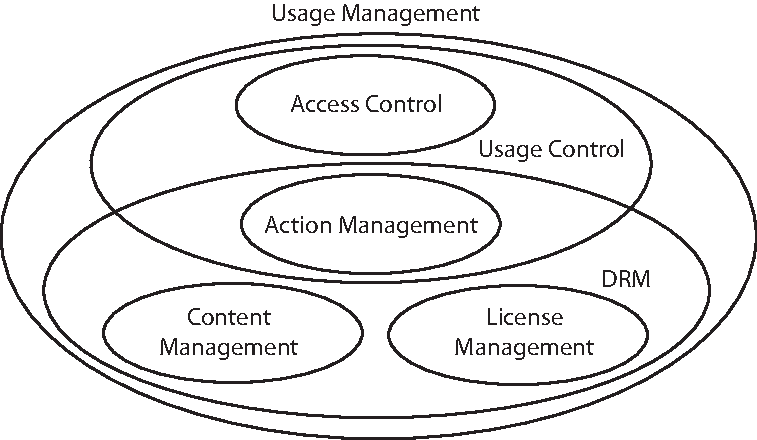
\includegraphics[width=3.75in]{./images/usage_management.pdf}}
%  \caption{The primary elements associated with a usage management system.}\label{UM}
%\end{figure}
%
%\emph{Access control} by itself is a rudimentary form of usage management that is concerned with mechanisms for determining what subjects may access a given set of objects under what conditions. Over the years, access control policy models and supporting languages have continued to evolve with increasing granularity in policy expression and sophistication in reasoning power~\cite{BlPa:76,HuFeKu:06}. Usage control is a relatively new concept that incorporates access as well as usage policies for users over resources~\cite{PaSa:04}. \emph{Usage control} mechanisms focus on access and subsequent usage of a resource over a finite period of time. Usage control models take into account semantics such as obligations and permissions. One of the important distinguishing features of usage control is usage tracking. \emph{DRM} includes license (or policy) management, content management, tracking, negotiation, rights expression languages, and payments~\cite{HeJaKhHr:07,JaHe:08b,JaHeMa:06}. In general, in DRM systems, the use of content objects is subject to the terms of a license~(policy), which is expressed using a REL. The last major component of a usage management system involves \emph{enforcement mechanisms}. These include software and/or hardware mechanism that may be used in an effort to enforce usage according to specified policy.
%
%These four areas form the components of a usage management system. A usage management system is thus capable of expressing complex, fine-grained usage policies over data elements and of ensuring subsequent interpretation, enforcement, and reasoning of these policies along with tracking of usage of those data elements in the computing environment. In this research, a usage management system will be developed specifically for the purpose of managing location-based policies and scenarios. 

%The current state-of-the-art in location services for mobile device divides into a few distinct categories. First, there is geolocation of mobile devices based upon their IP addresses. These approaches use tables of IP address ranges and other associated information to provide location services to subscribers via regional Internet registries~\cite{AIRN:13,RIPE:13}. This information can be retrieved via standard programming interfaces defined by the World Wide Web Consortium (W3C)~\cite{w3c:13}, and are supported by a variety of browser implementations ~\cite{firefox:13,Pi:13}. With this approach, developers use standard interfaces to retrieve information from Internet registries in order to locate individuals. This type of functionality exists for modern browsers on workstation-grade systems, as well as on most mobile platforms~\cite{opera:13,safari:13}.

%Another approach involves the use of dedicated GPS systems with network links. These types of systems are embodied by various platform mapping applications common on mobile platforms~\cite{amap:13,gmap:13}. Apple's iPhone, for example, currently offers assisted GPS services that use GPS information transmitted from satellites, as well as cellular and other network sources to locate devices~\cite{amap:13}. Though any of these systems can be used in device-to-device communication in a distributed Internet-of-things, GPS-equipped units are more common as they can provide finer levels of geolocation granularity.

%Finally, bringing this information together, there are data solutions such as those embodied by Google Earth and Esri %do not capitalize this!
%products such as ArcGIS~\cite{esri:13,gearth:13}. Both GPS-based and IP address-centric geolocation techniques can integrate with these types of data solutions into a single, unified system. With that in mind, however, these kinds of geographic information systems do not provide messaging functionality directly, nor do they implicitly support it---they can be leveraged as components to provide integrated solutions.

\sbirsection{Relationship with Future Research or Research and Development}{}
AHS Engineering Services was established to address the innovative application of information technologies. As a result, we are committed to the approach described in this proposal and are enthusiastic about its potential. Our current and past R\&D projects provide an excellent technical foundation for the Phase I effort. Phase I will demonstrate the feasibility of our approach and will lay the groundwork for the Phase II development and transition. Our Phase I work will rigorously show the covert channel characteristics of cross-domain workflows and establish the security bounds under which different protocols and classes of protocols can operate. Specifically, upon successful completion of Phase I, we will have analyzed a taxonomy of potential protocols and evaluated the most promising ones. With this information we will have prototyped reference implementations of the promising protocols and an example system facilitating cross-domain workflows. We will be well positioned to build production quality systems and supporting tools with rigorously verified covert communications characteristics, and we will have constructed a roadmap for application to an Air Force initiative within the Unified Cross Domain Management Office (UCDMO), which includes identifying the applicable clearances, certifications, and approvals required to conduct Phase II testing. Collectively, the anticipated results from Phase I will provide a solid foundation for Phase II. In Phase II, we will build the full WARDEN framework and apply it to the UCDMO. Phase III would bring this WARDEN framework to the marketplace (see Section~\ref{commercialization} below).

Our successful realization of our Phase I and II objectives and achievement of Phase III commercialization is expected to provide the following benefits to both Government and private sector customers of WARDEN:
\vspace{-0.1in}
\begin{itemize}
     \item Dynamically and securely share information when split between two security domains.
     \item An agile usage management framework that scales to the enterprise.
     \item Provides an information advantage to warfighters.
\end{itemize}

We are confident of our ability to successfully deliver these benefits. As for future R\&D, we will seek out ways to extend the scope of WARDEN to include more sophisticated policy-based usage management capabilities.

\sbirsection{Commercialization Strategy}{Our overall strategy for achieving technology transition and commercialization success will be to apply the WARDEN framework to the UCDMO while providing high return-on-investment to our Air Force transition customers.}
\label{commercialization}

\paragraph{Background.} As all aspects of science and society become increasingly information intensive, the need to understand, create, and apply new methods for modeling, managing, and acquiring information has never been greater. It is our mission to provide the structure necessary to handle the ever increasing amounts of data in the revolution of Information Security, Theory of Information, and Information Architecture through innovative research in order to securely manage the usage of information. The following subsections provide our market analysis and plans for commercialization of WARDEN.

\paragraph{Market Need and Size.} We have identified four key market segments to our plans for commercialization of WARDEN. Those market segments are social media, mobile communication, cloud computing, and big data, which are briefly described below. We intend to capitalize on the market timing generated by the current convergence of these four key market segments.

\vspace{-12pt}
\subparagraph{Social Media.} Social media refers to the means of interactions among people in which they create, share, and exchange information and ideas in virtual communities and networks. Social media may be defined as a group of Internet-based applications that build on the ideological and technological foundations of Web 2.0, and that allow the creation and exchange of user-generated content. Furthermore, social media depend on mobile and web-based technologies to create highly interactive platforms via which individuals and communities share, co-create, discuss, and modify user-generated content. It introduces substantial and pervasive changes to communication between organizations, communities, and individuals~\cite{WikipediaSocial:13}.
Internationally, revenue from social networks grew an estimated 43 percent year-over-year in 2012, putting the total amount of income generated by sites like Facebook, Twitter, and LinkedIn at \$16.9 billion. Gartner predicts social media revenue will reach \$34 billion by 2016, up from \$11.8 billion in 2011. Advertising and social gaming account for about 90 percent of total social revenue, says the information technology (IT) research and advisory company~\cite{Mi:12}.

\vspace{-12pt}
\subparagraph{Mobile Communication.} Mobile communication involves mobile hardware and mobile software. Hardware includes mobile devices or device components. Mobile software deals with the characteristics and requirements of mobile applications~\cite{WikipediaMobileComputing:13}. In addition to telephony, modern mobile phones also support a wide variety of other services such as text messaging, Multimedia Messaging Service (MMS), email, Internet access, short-range wireless communications (infrared, Bluetooth), business applications, gaming, and photography. Mobile smartphones offer these and more general computing capabilities~\cite{WikipediaMobilePhone:13}.
The market for mobile communication equipment grew by 13 percent in 2012, propelled by climbing shipments of mobile handsets and tablets, particularly devices supporting the 4G long term evolution (LTE) wireless standard. Total factory revenue from original equipment manufacturers making mobile communications equipment is projected to reach \$376 billion in 2012, up from \$334 billion in 2011, according to a report from information and analytics provider IHS. In 2013, overall revenue for mobile communication equipment is forecast to rise to \$444 million. Driven by mobile broadband, the five-year compound annual growth rate until 2016 will amount to 11 percent~\cite{Si:12}.

\vspace{-12pt}
\subparagraph{Cloud Computing.} Cloud computing is the use of computing resources (hardware and software) that are delivered as a service over a network. Cloud computing relies on sharing of resources to achieve coherence and economies of scale similar to a utility (like the electricity grid) over a network. At the foundation of cloud computing is the broader concept of converged infrastructure and shared services~\cite{WikipediaCloud:13}.
Recent IDC cloud research shows that worldwide revenue from public IT cloud services exceeded \$21.5 billion in 2010 and will reach \$72.9 billion in 2015, representing a compound annual growth rate of 27.6\%. This rapid growth rate is over four times the projected growth for the worldwide IT market as a whole (6.7\%). The cloud movement is about much more than the cloud. Cloud cannot be sufficiently understood as a standalone phenomenon in the IT market, but rather as a core ingredient of a larger transformation of the IT industry -- and many other industries using IT to transform themselves. Other ingredients enabled by cloud -- and, in turn, accelerating cloud adoption -- include the expanding "species" of mobile devices, the explosion of mobile apps, the growing availability of wireless broadband, and the explosion of big data tools~\cite{IDCCloud:13}.

\vspace{-12pt}
\subparagraph{Big Data.} Big data is a collection of data sets so large and complex that it becomes difficult to process using on-hand database management tools or traditional data processing applications. The challenges include capture, curation, storage, search, sharing, analysis, and visualization. The trend to larger data sets is due to the additional information derivable from analysis of a single large set of related data, as compared to separate smaller sets with the same total amount of data, allowing correlations to be found~\cite{WikipediaBig:13}.
IDC predicts that the market for big data technology and services will reach \$16.9 billion by 2015, up from \$3.2 billion in 2010. This represents a compound annual growth rate of 40\%, or about 7 times that of the overall information and communications technology market~\cite{IDCBig:13}.

\paragraph{Projected Commercialization Results.} Our commercialization strategy consists of two paths:
\begin{itemize}
  \item Our first path focuses on transitioning the technology to the UCDMO thereby providing direct return-on-investment for AFRL STTR investment. Our existing knowledge and experience working with the DIB will provide a solid foundation for success in this initiative.
  \item Our second path is deployment to other government customers and prime contractors, leveraging the WARDEN technology to address both known and anticipated needs they face in the area of assured information sharing.
\end{itemize}
The timeline and expected funding for commercialization are:
\vspace{-12pt}
\subparagraph{Year 1:} STTR Phase I funding of \$150,000 for concept feasibility and refinement. No additional capital expected.
\vspace{-12pt}
\subparagraph{Years 2--3:} STTR Phase II funding of \$1 million for concept development in the UCDMO (i.e., relevant environment). Anticipated additional customer capital of \$50,000--500,000 obtained to enhance the WARDEN design as a guard component.
\vspace{-12pt}
\subparagraph{Year 4:} STTR Phase III rollout of WARDEN, funded by customer capital raised according to needs. Anticipated customer capital of \$1--5 million obtained to provide protected communication and multi-domain coordination for a program of record (POR).

\sbirsection{Key Personnel}{AHS Engineering Services prides itself on teaming superbly qualified personnel for all of our projects. }\label{Key_Personnel}
All key personnel are United States citizens. We propose Dr. Mark Heileman, Dr. Gregory Heileman, and Dr. Christopher Lamb as Phase I Co-Principal Investigators. Dr. Mark Heileman's biography and r\'esum\'e are below. Dr. Gregory Heileman's biography and r\'esum\'e are in Section~\ref{subs}. Dr. Lamb's biography and r\'esum\'e are in Section~\ref{subs}.
\vspace{-0.1in}
\begin{center}
   \fcolorbox{BlueSteel}{Magnum}{
         \begin{minipage}[t]{0.9\textwidth}
             \begin{itemize}[labelindent=2em,leftmargin=1.5em,label=$\checkmark$] 
  		\item Dr. Mark Heileman has extensive experience as a research engineer and software system developer. He has focused on applying advanced information technology and modeling to solve real-world business problems.
  		\item Dr. Gregory Heileman is a recognized leader in machine learning and directs the Informatics Lab at the University of New Mexico where he is Associate Provost and Professor in the Department of Electrical and Computer Engineering.
		\item Dr. Christopher Lamb  is a TOGAF certified enterprise architect and a Certified Information Systems Security Professional. An experienced software engineer, he is actively engaged in cyber-security research as well, focusing specifically on distributed content network topologies, usage management, and cloud computing.
 	\end{itemize}
         \end{minipage}
      }
\end{center}

\vspace{-6pt}

{\bfseries Co-Principal Investigator. Dr. Mark Heileman} is a Research Manager at AHS Engineering Services. Dr. Heileman's over thirty-year career includes engineering and executive positions with Modus Operandi, Elisar Software Corporation, i2 Technologies, United Space Alliance, Rockwell International, and Harris Corporation. His mission is to focus on the client's challenges and employ a consultative, systems engineering approach to solve complex business needs. Dr. Heileman is a graduate of the University of Central Florida where he earned a Ph.D. in Industrial Engineering and Management Systems. He is a registered professional engineer in Florida.

\textbf{\textsc{Mark D. Heileman \hfill Research Manager}}

\vspace{-18pt}
{\textcolor{black}{\makebox[6.5in]{\hrulefill}} 
\textbf{\textsc{Technical Expertise:}}
\vspace{-8pt}
\begin{multicols}{2}
 \begin{itemize}
  \item Enterprise Information Systems
  \item Digital Rights Management
  \item Cyber Security
  \item Expert Systems
  \item Data Aggregation
  \item Simulation and modeling	
 \end{itemize}
\end{multicols}
\vspace{-16pt}
\textbf{\textsc{Selected Publications:}}
\vspace{-8pt}
\begin{enumerate}
\item M. Heileman, G. Heileman, M. Shaver, P. Jamkhedkar, and M. Gilger. SMASHUP: Secure Mashup for Defense Transformation and Net-Centric Systems. Prepared for SPIE Defense, Security, and Sensing 2011 Conference, Orlando, FL, 25--29 April 2011.
\item G. Heileman and M. Heileman. Method and Apparatus for Integrating Subjective Trust Measures into Automated Decision-Making Processes. Provisional Patent Application, USA, submitted 19 May 2010.
\item M. Heileman, G. Heileman, and J. Hwang. Integrating Subjective Trust into Networked Infrastructures. Prepared for Systems \& Software Technology Conference (SSTC) 2009, Salt Lake City, UT, 20--23 April 2009.
\item R. Hull, K. Bimson, M. Heileman, R. Hyle, and R. Thiebauth. Semantic Service-Oriented Architecture for Range Operations: Evolving the Role of Semantics in the Enterprise. Prepared for SPIE Defense, Security, and Sensing 2009 Conference, Orlando, FL, 13--17 April 2009.
\item H. Goldstein, G. Heileman, M. Heileman, et al. Protecting Digital Archives at the Greek Orthodox Archdiocese of America. Prepared for DRM'03, Washington, DC, 27 October 2003.
\item D. Linton, S. Khajenoori, M. Heileman, J. Bullington, H. Cat, K. Halder, G. Hebert, and S. Sinnappan. ``Reporter Object: An Analysis Module Which Aids in Verifying, Validating and Graphically Displaying Results of Simulation Models,'' Simulation, Vol. 62, No. 5, May 1994, pp. 313--328.
\item M. Heileman, D. Linton, and S. Khajenoori. ``Simulation Study Aids Space Shuttle Flight Rate Planning,'' Industrial Engineering, Vol. 24, No. 3, March 1992, pp. 58--59.
\end{enumerate}

\vspace{-6pt}
\textbf{\textsc{Relevant Experience:}}~\\
{\bfseries AHS Engineering Services, 2013--present. Research Manager.} A research and development firm offering expert engineering services in areas including software engineering and information security.~\\
{\bfseries Modus Operandi, Inc., 2004--2013. Scientist.} A software company serving the US defense and intelligence community by providing technology to speed information discovery, integration, and fusion. Directed the design and development of innovative information system technologies and their application to government and industry needs.~\\
{\bfseries Elisar Software Corporation, 2001--2003. Vice President, Sales Engineering.} A venture capital financed start-up software company providing digital rights enforcement products and services. Initiated the Sales Engineering function, which had primary responsibility for driving customer and market requirements into the internal development process.~\\
{\bfseries i2 Technologies, 1997--2001. Senior Solution Consultant}. A business software and services company providing supply chain management solutions to customers worldwide. Provided technical leadership throughout software products sales cycles.

\vspace{-6pt}
\textbf{\textsc{Education:}}
\vspace{-30pt}
\begin{tabbing}*****************\=\kill
 \> {\bfseries Ph.D.}, Industrial Engineering \& Management Systems, Univ. of Central Florida (1997). \\
 \> {\bfseries M.S.}, Engineering Management, Florida Institute of Technology (1990). \\
 \> {\bfseries M.B.A.}, Business Administration, Florida Institute of Technology (1985). \\
 \> {\bfseries B.S.}, Industrial and Systems Engineering, University of Florida (1980).
\end{tabbing}

\vspace{-12pt}
\textbf{\textsc{Affiliations:}}
\vspace{-30pt}
\begin{tabbing}*****************\=\kill
\> Registered Professional Engineer, State of Florida (P.E. \#35539). \\
\> Senior Member, Institute of Industrial Engineers. \\
\> Member, International Council on Systems Engineering (INCOSE). \\
\> Security Clearance: DoD Top Secret/SCI.
\end{tabbing}
\vspace{-12pt}

\sbirsection{Foreign Citizens}{}
We do not expect to involve any foreign citizens on this project.

\sbirsection{Facilities/Equipment} {}
All instrumentation and physical facilities required to carry out the Phase I effort are available at AHS Engineering Services and the University of New Mexico facilities in Albuquerque, NM. All project key personnel have dedicated laptop computers with high-speed network connection. No items of equipment are to be purchased for the Phase I effort. These facilities meet all environmental laws and regulations of federal, New Mexico, and local governments for, but not limited to, the following groupings: airborne emissions, waterborne effluents, external radiation levels, outdoor noise, solid and bulk waste disposal practices, and handling and storage of toxic and hazardous materials.

\sbirsection{Subcontractors/Consultants}{Dr. Gregory Heileman and Dr. Chris Lamb are uniquely qualified for this effort, and their active involvement will ensure the success in delivering value to the Air Force Research Laboratory.}\label{subs}

\subsection{University of New Mexico Key Personnel}\label{AHS}

{\bf Co-Principal Investigator. Dr. Gregory Heileman } is the Associate Provost for Curriculum and a Professor in the Department of Electrical and Computer Engineering at the University of New Mexico, with over 20 years of experience as a research scientist, and over 100 peer-reviewed journal articles and conference papers. At the University of New Mexico he teaches courses in the areas of algorithms and data structures, software design, theory of computing, learning theory, and information theory. His research interests are in the areas of information security and multimedia systems, the theory of computing and information, and machine learning. He currently serves on the Editorial Board for the International Journal of Multimedia Intelligence and Security. He is the author of the textbook Data Structures, Algorithms, and Object-Oriented Programming published by McGraw-Hill in 1996. During 1998 he held a research fellowship at the Universidad Carlos III de Madrid, and in 2005 he held a similar position at the Universidad Polit\'enica de Madrid. Dr. Heileman is a senior member of the IEEE. He holds a PhD in Computer Engineering from the University of Central Florida.

\textbf{\textsc{Gregory L. Heileman \hfill Professor and Associate Provost}}

\vspace{-18pt}
{\textcolor{black}{\makebox[6.5in]{\hrulefill}} 
\textbf{\textsc{Technical Expertise:}}
\vspace{-8pt}
\begin{multicols}{2}
 \begin{itemize}
  \item Machine Learning
  \item Usage Management
  \item Information Security
  \item Data Structures and Algorithmic Analysis
  \item Theory of Computing and Information	
 \end{itemize}
\end{multicols}

\vspace{-16pt}
\textbf{\textsc{Selected Publications:}}
\vspace{-8pt}
\begin{enumerate}
\item C.~C. Lamb and G.~L. Heileman. Content-centric Information Protection in the Cloud, {\sl International Journal of Cloud Computing and Services Science  (IJ-CLOSER)}, 2(1):246-257, 2013.
\item P. A. Jamkhedkar, C. C. Lamb, and G. L. Heileman. Usage Management in Cloud Computing, In F. Hartung, T. Kalker and S. Lian, Eds., {\sl Digital Rights Management: Technology, Standards and Applications}, Auerbach Publications, 2012. 
\item C. C. Lamb, P. A. Jamkhedkar, G. L. Heileman and C. T. Abdallah. Managed Control of Composite Cloud Systems. 6th IEEE International Conference on System of Systems Engineering (SoSE), Albuquerque, NM, pp. 167--172, June 27--30, 2011.
\item P.~A. Jamkhedkar and G.~L. Heileman. Rights Expression Languages, in S. Lian and Y. Zhang, Eds., {Handbook of Research on Secure Multimedia Distribution}, IGI Global, Hershey, PA, 2008. 
\item S. al-Saffar and G. L. Heileman. Computing Information Value from RDF Graph Properties. Proceedings of the 12th International Conference on Information Integration and Web-based Applications \& Services, Paris, Nov. 8--10, 2010.
\item T.-T. Quach F. Perez-Gonzalez, and G. L. Heileman. Model-Based Steganalysis Using Invariant Features. IS\&T/SPIE Electronic Imaging Science and Technology: Media Forensics and Security XI (Conference EI120), San Jose, CA, Jan. 18--22, 2009.
\item S. al-Saffar and G. L. Heileman. Semantic Impact Graphs for Information Valuation. Proceeding of the Eighth ACM Symposium on Document Engineering, Sao Paulo, Brazil, pp. 209--212, Sept. 16--19, 2008.
\item S. al-Saffar and G. L. Heileman. Semantics-Based Information Valuation. Proceedings of the 4-th IEEE International Conference on Intelligent Systems IS'08, Varna, Bulgaria, Vol. 1, pp. 6-51--6-58, Sept. 6--8, 2008.
\end{enumerate}

\vspace{-6pt}
\textbf{\textsc{Relevant Experience:}}~\\
{\bfseries AHS Engineering Services, 1997--present. Principal.} A research and development firm offering expert engineering services in areas including software engineering and information security.~\\
{\bfseries University of New Mexico, Department of Electrical \& Computer Engineering, 1990--present. Professor, Associate Provost for Curriculum (current position)}.~\\
{\bfseries Elisar Software Corporation, 2000--2003. Chief Executive Officer and Chairman of the Board.} A venture capital financed start-up software company providing digital rights enforcement products and services.

\vspace{-6pt}
\textbf{\textsc{Education:}}
\vspace{-30pt}
\begin{tabbing}*****************\=\kill
 \> {\bfseries Ph.D.}, Computer Engineering, University of Central Florida (1989). \\
 \> {\bfseries M.S.}, Biomedical Engineering \& Mathematics, University of North Carolina (1986). \\
 \> {\bfseries B.A.}, Biology, Wake Forest University (1982).
\end{tabbing}

\vspace{-12pt}
\textbf{\textsc{Affiliations:}}
\vspace{-30pt}
\begin{tabbing}*****************\=\kill
\> Editorial Board,  International Journal of Multimedia Intelligence and Security. \\
\> Senior Member, IEEE. \\
\> Security Clearance: DoD Secret.
\end{tabbing}
\vspace{-12pt}

\subsection{Sandia National Laboratories Key Personnel}

{\bf Co-Principal Investigator. Dr. Christopher Lamb} will act as the primary Systems Architect during the course of all phases of the project. Dr. Lamb currently serves as an Enterprise Architect, with concentration on Systems and Security, with Sandia National Laboratories. He is also a research professor affiliated with the Electrical and Computer Engineering department at the University of New Mexico. He has extensive experience designing and developing mission-critical distributed systems for a wide range of government departments and agencies. Prior to joining Sandia National Laboratories, Dr. Lamb served in executive roles and as a principal consultant for a variety of technology companies in the southwest. Dr. Lamb has a B.S. in Mechanical Engineering from New Mexico State University, an M.S. in Computer Science from the University of New Mexico, as well as a Ph.D. in Computer Engineering with a focus on Computational Intelligence from the University of New Mexico. He is a The Open Group Architecture Framework (TOGAF) 9 Certified Enterprise Architect and a Certified Information Systems Security Professional (CISSP) through the International Information Systems Security Certification Consortium.

\textbf{\textsc{Christopher C. Lamb \hfill Research Professor / Principal Scientist}}

\vspace{-18pt}
{\textcolor{black}{\makebox[6.5in]{\hrulefill}} 
\textbf{\textsc{Technical Expertise:}}
\vspace{-8pt}
\begin{multicols}{2}
 \begin{itemize}
  \item Cloud Systems Security
  \item Usage Management
  \item Systems and Software Architecture
  \item Software Engineering and Design
  \item Next-Generation Software Systems Security	
 \end{itemize}
\end{multicols}

\vspace{-16pt}
\textbf{\textsc{Selected Publications:}}
\begin{enumerate}
\item Christopher Lamb and Gregory Heileman.
\newblock Content-centric information protection in cloud computing.
\newblock {\em International Journal of Cloud Computing and Services Science},
  2(1):246--257, 2012.

\item Christopher~C. Lamb, Pramod~A. Jamkhedkar, and Gregory~L. Heileman.
\newblock {\em Digital Rights Management: Technology, Standards and
  Applications}.
\newblock Auerbach Publications, 2013.

\item C.C. Lamb and G.L. Heileman.
\newblock Overlay architectures enabling cloud computing for multi-level
  security environments.
\newblock In {\em Services (SERVICES), 2012 IEEE Eighth World Congress on},
  pages 116 --124, june 2012.

\item Christopher~Charles Lamb, Pramod~A. Jamkhedkar, Mathew~P. Bohnsack, Viswanath
  Nandina, and Gregory~L. Heileman.
\newblock A domain specific language for usage management.
\newblock In {\em Proceedings of the 11th annual ACM workshop on Digital rights
  management}, DRM '11, pages 51--62, New York, NY, USA, 2011. ACM.

\item Christopher~C. Lamb, Pramod~A. Jamkhedkar, Gregory~L. Heileman, and Chaouki~T.
  Abdallah.
\newblock Managed control of composite cloud systems.
\newblock In {\em System of Systems Engineering (SoSE), 2011 6th International
  Conference on}, pages 167 --172, june 2011.

\item P.A. Jamkhedkar, C.C. Lamb, and G.L. Heileman.
\newblock Usage management in cloud computing.
\newblock In {\em Cloud Computing (CLOUD), 2011 IEEE International Conference
  on}, pages 525 --532, july 2011.

\item Pramod~A. Jamkhedkar, Gregory~L. Heileman, and Chris~C. Lamb.
\newblock An interoperable usage management framework.
\newblock In {\em Proceedings of the tenth annual ACM workshop on Digital
  rights management}, DRM '10, pages 73--88, New York, NY, USA, 2010. ACM.
\end{enumerate}

\vspace{-6pt}
\textbf{\textsc{Relevant Experience:}}~\\
{\bfseries Sandia National Laboratories, 2004--present. Principal Scientist.} Architecture development and security analysis; ICAM architectures; heterogeneous analytic component systems engineering; program development; micro-controller engineering (PIC32, PIC16); service-oriented system architecture, design, and development; software engineering; general project management.~\\
{\bfseries Oso Grande Technologies, 2001--2004. Vice President, Software Engineering.} Led a multi-disciplinary team brokering information via web services between national insurance aggregators and state governments; responsible for profitability, business development, technical architecture and development.

\vspace{-6pt}
\textbf{\textsc{Education:}}
\vspace{-27pt}
\begin{tabbing}*****************\=\kill
 \> {\bfseries Ph.D.}, Computer Engineering, University of New Mexico (2012). \\
 \> {\bfseries M.S.}, Computer Science, University of New Mexico (2002). \\
 \> {\bfseries B.S.}, Mechanical Engineering, New Mexico State University (1994).
\end{tabbing}

\vspace{-12pt}
\textbf{\textsc{Affiliations:}}
\vspace{-27pt}
\begin{tabbing}*****************\=\kill
\> Member, IEEE. \\
\> Security Clearance: DoE Q.
\end{tabbing}
\vspace{-12pt}

\sbirsection{Prior, Current, or Pending Support of Similar Proposals or Awards}{}
No prior, current, or pending support for the proposed work.

{
%\small
 \bibliography{proposal}
 \bibliographystyle{abbrv}
 }
 
\end{document} 